\chapter{Recommendations}
\label{cha:recommendations}

This chapter makes several recommendations to the client for future work on the
delivered product. First, recommendations are made to improve the REPL backend
itself. Secondly, suggestions are made on how to improve the Eclipse frontend.
Finally, a recommendation is made to provide literate programming functionality.

\section{Extending the functionality of the REPL}
\label{sec:impr-backend}

The delivered backend is a solid product. Due to time constraints, however, some
desirable features have not been implemented. This subsection shortly highlights
these features.

\subsubsection{More extensive history functionality}

The current input history implementation provides a means of iterating the
previously entered expressions in a linear way: a user can scroll back and forth
through the old entries. It would be nice if the history was searchable, too.
When implementing this, one could turn to existing command-line shells for
inspiration. The GNU readline library, for example, has two ways of searching
through the input history: via a keyboard shortcut, which when pressed allows
the user to enter a word that they remember is in the entry they are looking
for, or via an always-on setting that allows the user to enter the beginning of
the expression which will in turn filter the linear iteration over the
history to only those entries starting with the entered input.

Another limitation of the current history implementation is the fact that it is
recorded per session. This means that when a user uses several languages in the
same session, the history will contain entries from both languages. Instead,
history should perhaps be kept not only per session, but also per language.

Related to the above, is implementing persistent history. The Eclipse frontend
currently only provides volatile history, which means that history is thrown
away when Eclipse is closed. The console plugin does provide persistent history,
but this implementation also leaves things to be desired: all history is saved
into the same file, resulting again in a mixed history. The recommendation that
is made here is to provide the ability to have separate, per language
persistent history. If the frontend is an IDE, these files can perhaps be saved
inside the language project's directory structure.

Improving the history implementation should result in a smoother and
faster way to interact with the REPL, enhancing the explorative nature.

\subsubsection{Analysis in context}

%%% Local Variables:
%%% mode: latex
%%% TeX-master: "../main"
%%% End:


\subsubsection{Adding support for alternative evaluation strategies}
\label{ssec:discuss-alternate-eval}

As discussed in \cref{sec:eval-strat}, languages developed with Spoofax are not
limited to a single interpreter. Instead, there can be different strategies for
evaluation. While this has been taken into account for the design of the
product, only a DynSem evaluation strategy has actually been implemented.

Languages with a Java backend (such as IceDust%
\footnote{https://github.com/MetaBorgCube/IceDust}) therefore do not currently
work with the REPL. To add support for specific interpreters, a language should
provide the REPL with a named implementation of the
\texttt{``IEvaluationStrategy''}. The language designer can register alternative
evaluation strategies with the REPL by extending the Guice module of the backend
and overriding the \texttt{bindEvalStrategies} method.

Finally, the evaluation strategy that will be used to evaluate input terms can
be configured via the ShellFacet ESV extensions (see \cref{sec:esv-extensions})
as illustrated in \cref{lst:eval-method}.

\begin{lstlisting}[language=esv,caption={Setting the evaluation strategy.},label={lst:eval-method}]
module editor/SL-Shell

shell
    evaluation method : "dynsem"
\end{lstlisting}



\section{Improvements to the Eclipse frontend}
\label{sec:impr-eclipse}

\section{Eclipse Multithreading Issues}
\label{sec:eclipse-multithread}

The implementation of the Eclipse frontend has been a source of exposing many
shortcomings in the initial designs. These shortcomings and how they have been
resolved are discussed in this section.

\subsection{Single- versus multithreading}

The initial design assumed that the frontends and the backend would run in the
same thread. For a console based REPL, this assumption holds and greatly
simplifies the design. However, this assumption does not hold when the backend
has a frontend using a multithreaded GUI toolkit. This
assumption resulted in two problems, which are listed separately in the next
sections. The solution and changes made to the design are then discussed
afterwards.

\subsection{Blocking- versus non-blocking input}

In a multi-threaded environment, asking graphical text entry widgets for the
entered text is rarely a blocking process. The REPL backend at the time,
however, assumed that getting the user's input was always a blocking operation.
Therefore, when a conceptual Eclipse frontend was made, the REPL spun into an
infinite loop trying to execute empty expressions.

\subsection{Evaluating on the UI thread}

As explained in \cref{ssec:eclipse-plugin}, multi-threaded graphical user
interface toolkits often use multiple threads. One of these threads is
designated the ``UI thread'', or user interface thread. This thread is
responsible for processing events (such as mouse clicks) and updating the
graphical representation of the widgets. All tasks that perform long running
calculations are supposed to be run in a background thread, such that the UI
thread is free to process incoming events. Instead, if a long running
computation is run in the UI thread, the widgets on the screen stop responding
to the user and the program appears to be in a frozen state. This is exactly
what happened when the backend assumed to be run in the same thread as the
frontend: whilst the backend was evaluation expressions, Eclipse appeared to be
frozen due to this evaluation taking place in the UI thread from which the
execution was started. This issue would be worse in case blocking input
were to be used.

\subsection{Accustoming to multi-threaded frontends}

As indicated in the previous sections, the only solution to these problems is to
allow multi-threaded frontends. This meant that the assumption of every
operation running in the same thread no longer held. As a result, several
changes had to be made:

\begin{enumerate}
  \item Initially, a \texttt{``Repl''} class was present in the backend to
  centralize a REPL implementation. This class made too many assumptions on
  behalf of the frontends, among which blocking user input and the entire main
  loop of a REPL. The alternative is the \texttt{``IRepl''} interface (see
  \cref{sec:overview}), which defines the only method each frontend has in
  common: the \texttt{eval} method to evaluate input. It is now entirely up to
  the frontend on how to implement the read, print and loop steps, allowing for
  much more freedom.
  \item	The initial design provided ``hooks'' to the frontend to process results or
  errors. A frontend would register itself to process certain hooks, after which
  the registered method would be called. The registered methods would be called
  immediately after the evaluation was done, and on the same thread. In the
  conceptual Eclipse frontend, these hooks updated the widgets running in the UI
  thread. This then led to widgets being updated from a thread other than the UI
  thread. The solution, discussed in \cref{sec:visitor}, was to return the
  result to the frontend, allowing it to process the result whenever and however
  it needs.
\end{enumerate}

Not only did these changes resolve the threading issues, they also made for a
cleaner architecture overall. An additional advantage is that a much wider scala
of possible frontends is now supported.

%%% Local Variables:
%%% mode: latex
%%% TeX-master: "../main"
%%% End:


\section{An IPython kernel for Jupyter notebooks}
\label{sec:discuss-literate-programming}

\section{Literate Programming}
\label{sec:literate-programming}

Just as with REPLs, the concept of literate programming is implemented in
various forms under various names. Therefore, this section starts with an
explanation of what literate programming is based on a few implementations.
Afterwards, the IPython implemention of literate programming is explored in more
detail.

Literate programming, as defined by Donald Knuth~\cite{knuth1984}, introduces
the ability to annotate source code with natural language. According to Knuth,
better documentation of programs is essential to make further progress in the
state of the art of programming.  To achieve this he proposes to write programs
not with the intention to explain the computer what to do, but with the
intention to explain to humans what the programmer wants a computer to
do~\cite{knuth1984} by mixing documentation and source code in a single file.
This idea of literate programming was realized in its original form as the
``WEB'' language developed during Knuth's research at Stanford University.

Even though the idea was conceived over thirty years ago, implementations are not
very common. However, in recent years the idea seems to gain popularity again.
A very recent implementation of literate programming is Apple's Swift
playgrounds~\cite{swift-playgrounds}. Swift playgrounds are interactive
documents or ``notebooks'' in which code is executed as it is typed, in
contrast to the non-interactive style of the ``WEB'' language in which \TeX{} and
PASCAL were combined into one language: \TeX{} served to document the program
and PASCAL to produce a machine-executable program.

In recent years, there has also been a particular focus on reproducible
research. While literate programming primarily aims to add documentation to
code, reproducible research focuses on adding code to documentation. More
specifically, reproducible research refers to the idea that scientific papers
should be augmented with the computer code used to carry out the
research~\cite{schulte2012}. Examples of recent projects claiming to support
both reproducible research and literate programming include the IPython
project~\cite{ipython2007} and Emacs Org-mode~\cite{schulte2012}.

\subsubsection{IPython with Jupyter notebooks}

IPython, together with Jupyter notebooks,
supports both reproducible research and literate programming. IPython was
partially inspired by other scientific tools already offering notebook-like
functionality, such as Matlab or Mathematica. Since its inception, the project
has been split off into IPython, which provides an interactive REPL and a
kernel that runs the user's code, and Jupyter notebooks, which provide the
notebook format and web application. Like Swift playgrounds, Jupyter notebooks
allow for REPL-style interactive editing; documentation and code can be edited
live and blocks of code can be reevaluated, printing their updated results.
Jupyter notebooks also allow for more complex graphical elements such as
3D-plots. See \cref{fig:ipython} for an example of an IPython notebook.

\begin{figure}[htb]
  \centering
  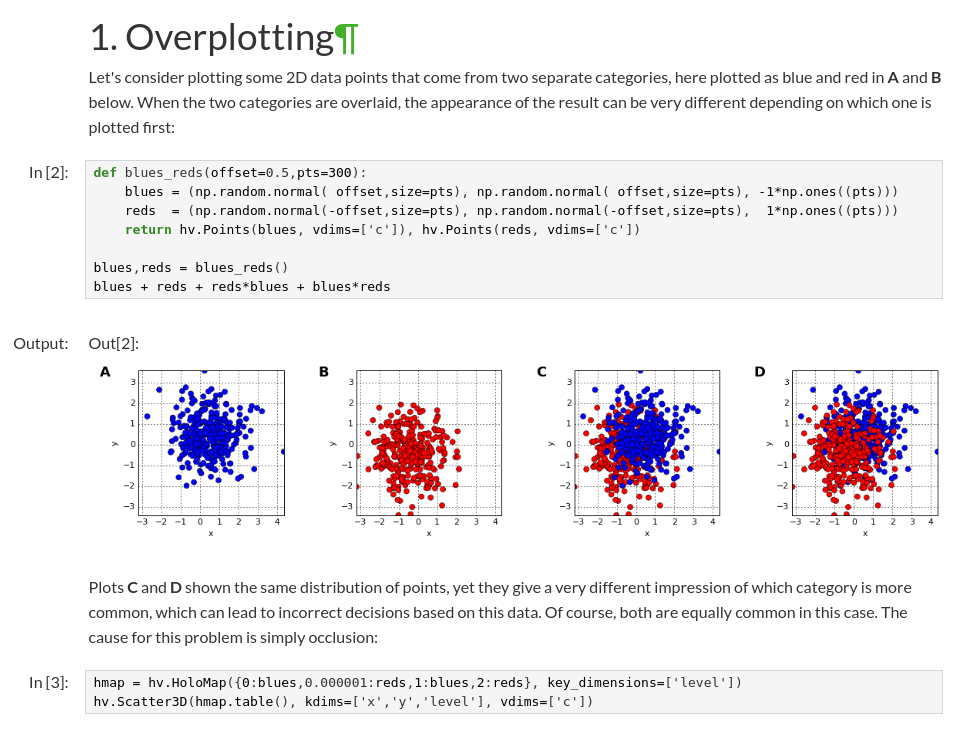
\includegraphics[width=\textwidth]{ipython}
  \caption{A plot from data in an IPython notebook.}
  \label{fig:ipython}
\end{figure}

As explained, IPython and Jupyter notebooks have become more or less separate
projects, to the extent that Jupyter notebooks can use several kernels.
Nowadays there are kernels for over forty languages that can be used in these
notebooks. This illustrates that in Python's case literate programming is more
or less an extension to the interactive IPython REPL. Since Jupyter notebooks
reuse the IPython REPL, the execution model used for Jupyter notebooks is
essentially the same as it is for IPython~\cite{ipython-execution}.

%%% Local Variables:
%%% mode: latex
%%% TeX-master: "../main"
%%% End:


%%% Local Variables:
%%% mode: latex
%%% TeX-master: "main"
%%% End:
